\documentclass{article}
\usepackage{graphicx}
%permite ecribir acentos directamente
\usepackage[utf8]{inputenc}
% Esto es para que el LÁTEX sepa que el texto está en español, se agrega el ingles para el paquete de gráfico de circuitos:
\usepackage[spanish]{babel}

\usepackage{geometry}
 \geometry{a4paper,total={170mm,257mm},left=15mm,right=15mm,top=20mm,}
 
\usepackage{amsmath, amsfonts}
\usepackage{enumitem}
\usepackage{xcolor}
\usepackage{textcomp}
 
\begin{document}

\begin{titlepage}
 \centering
	
\includegraphics[scale=0.80]{imagenes/LOGO.jpg} \par
 	\vspace{1cm}
 	{\scshape\LARGE Universidad Tecnológica Nacional \par}
 	{\scshape\large Facultad Regional de Córdoba \par}
 	\vspace{1cm}
	{\bfseries \Large Trabajo Práctico De Laboratorio $N^{\circ} 2$\par}
	{\bfseries \Large Control de ángulo de conducción de un SCR \par}
 	\vspace{1.5cm}

	\begin{tabular}{ll}
		Alassia, Francisco	&	60861	\\
		Amaya, Matías		&	68284	\\
		Lamas, Matías 		&	65536 	\\
		Navarro, Facundo 	&	63809 	\\
		Veron, Misael	 	&	62628
	\end{tabular}
	
	\vspace{1cm}
	Curso: 5r2 \\
	Grupo $N^{\circ} 11$
 	\vfill
	{\bfseries \Large Electrónica de Potencia \par}

	\vspace{1.5cm}
	Docentes: \par
	Ing. Oros \par
	Ing. Rabinovich \par

 	\vfill
	{\large \today\par}
\end{titlepage}

%##################################### INDICE  #####################################################

\tableofcontents
\clearpage

%##################################### INDICE  #####################################################

\section{Introducción}
Diseñar y construir un circuito para el control del ángulo de conducción de un SCR mediante el método escalón-rampa coseno. La tensión en la carga debe ser controlada por una señal de reverencia $V_{reff}$ , que variará entre 0 y 10 $V$.


\subsection{Funcionamiento}
La figura \textcolor{blue}{\ref{fig:fig1}} al circuito de control del ángulo de conducción de onda completa de un SCR con disparo por UJT. El circuito del método escalón-rampa coseno de la figura \textcolor{blue}{\ref{fig:fig2}}  , deriva del circuito anterior con el agregado de algunas variantes que permite mayor linealidad entre la tensión de referencia y la tensión en la carga.

\begin{figure}[h]
 \begin{center}
	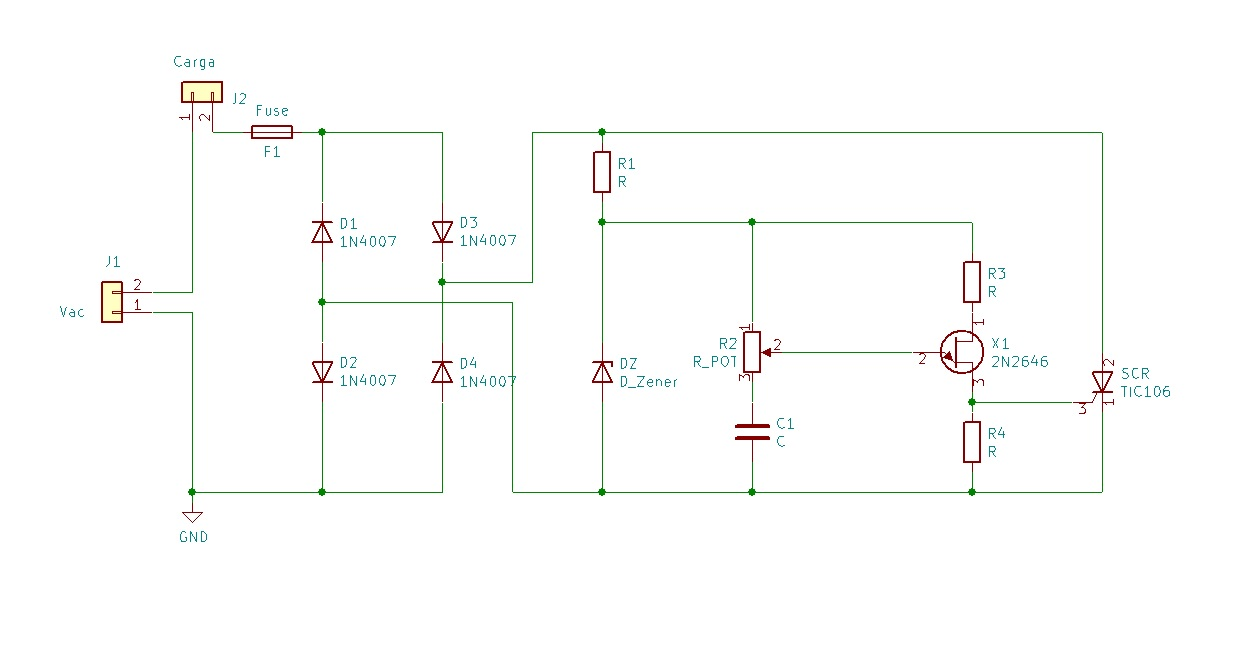
\includegraphics[scale=0.7]{imagenes/fig1.jpg} 
	\caption{Control de ángulo de conducción de un SCR por un UJT}\label{fig:fig1}
 \end{center}
\end{figure}

Cuando $V_C1$ se iguala a la tensión $V_P$ (disparo del unijuntura), éste se dispara y genera un impulso de corriente entre sus bases que, a su vez produce el disparo del SCR.

\begin{figure}[h]
 \begin{center}
	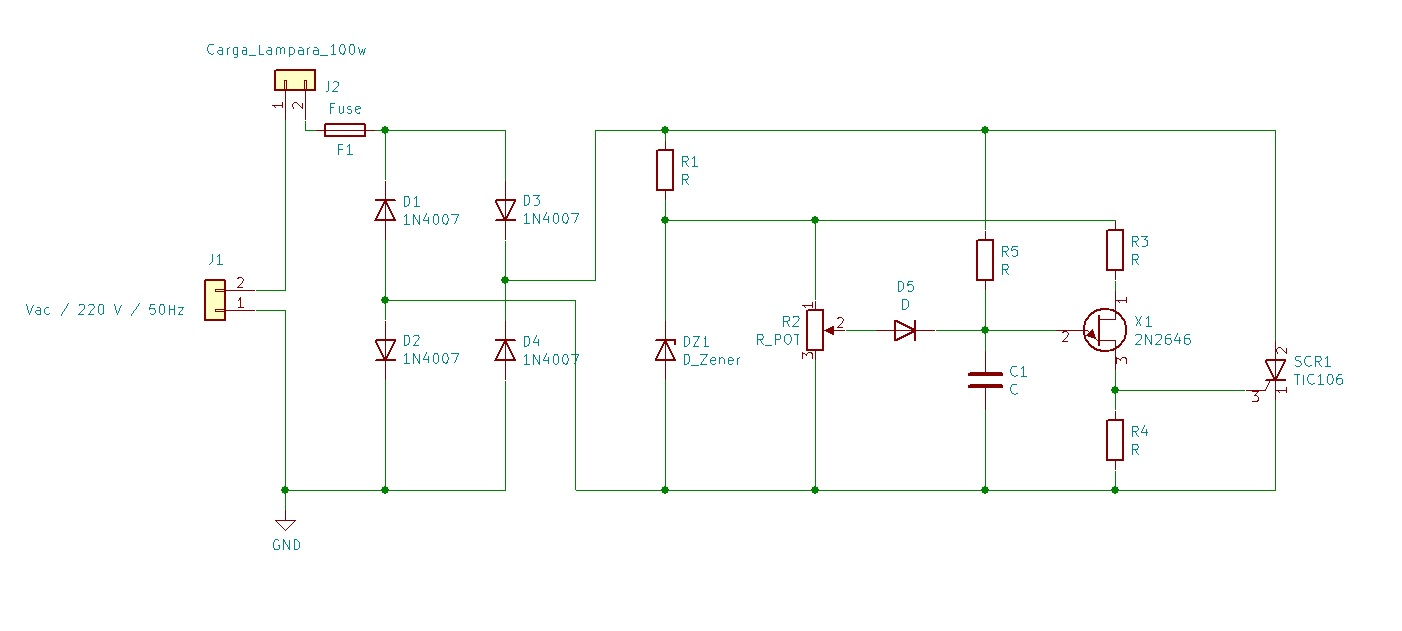
\includegraphics[scale=0.6]{imagenes/fig2.jpg} 
	\caption{Circuito escalón-rampa coseno}\label{fig:fig2}
 \end{center}
\end{figure}

El método escalón-rampa consiste en cargar el capacitor con un escalón inicial de amplitud variable (malla $R_2$ - $D_5$ - $C_1$) y luego con una rampa de pendiente fija (rama $R_5$ - $C_1$). El capacitor se carga inicialmente a través de la resistencia del potenciómetro $R_2$ y del diodo $D_5$. Una vez cargado con el escalón inicial, el diodo deja de conducir y el capacitor pasa a cargarse con la tensión rectificada de la línea a través de $R_5$ hasta que $V_{C1}$ se iguala a la tensión $V_P$ produciendo el disparo del UJT.

La malla $R_2$ - $D_5$ - $C_1$ se define como constante de tiempo $\tau_1$ y la rama $R_5$ - $C_1$ como $\tau_2$, siendo el valor de la misma mucho mayor que $\tau_1$ de forma que la tensión en el capacitor forme una rampa. El valor de esta constante $\tau_2$ debe satisfacer el caso de que el escalón inicial sea nulo (el potenciómetro en su extremo inferior), para que la tensión en el capacitor llegue a la tensión de disparo ($10 V$) en un semiciclo de la tensión de entrada.

Si se modifica la rampa de forma que su crecimiento no sea lineal, sino cosenoidal, se logra que la tensión de referencia $V_C$ (tensión instantánea en el capacitor) y la tensión aplicada en la carga $V_L$, sea prácticamente lineal.

El puente de diodos $D_1$-$D_4$, son los encargados de rectificar la tensión de línea para el correcto funcionamiento del SCR. $R_1$ limita la corriente que circuila por el diodo zener.
%
\section{Desarrollo}
Para el diseño, los dispositivos elegidos son los siguientes:
\begin{itemize}\itemsep0em \itemindent=2em
	\item[•]{\makebox[0.9cm]{SCR\hfill}: TIC 106}
	\item[•]{\makebox[0.9cm]{UJT\hfill}: 2N2646}
	\item[•]{\makebox[0.9cm]{Zener\hfill}: 1N4745}
	\item[•]{\makebox[0.9cm]{Diodo\hfill}: 1N4007}
\end{itemize}
%
\subsection{Cálculos}
Por consigna, debe efectuarse para una carga resistiva de $220\;V_{RMS}$ y $1\;kW$, entonces
\begin{align*}
	I_L &= \frac{P_L}{V_L} \\
	I_L	&= \frac{1000\;W}{220\;V_{RMS}} \\
	I_L	&= 4,54 \; A_{RMS}
\end{align*}

De la hoja de datos del SCR, se tiene:
%
\begin{itemize}\itemsep0em \itemindent=2em
	\item[•]{\makebox[1cm]{$V_{DRM}$\hfill}= $400 \; V$}
	\item[•]{\makebox[1cm]{$I_T$\hfill}= $5 \; A$ a 80\textdegree{C}}
	\item[•]{\makebox[1cm]{$I_{GT}$\hfill}= $200 \; \mu A$}
	\item[•]{\makebox[1cm]{$V_{GT}$\hfill}= $1,2 \; V$}
\end{itemize}
Para garantizar que el disparo se encuentre siempre dentro de la zona de disparo seguro, se establece:
\begin{align*}
	I_G &= 5 * I_{GT} \\
	I_G	&= 1 \; mA
\end{align*}
%
De la hoja de datos del UJT, se tiene:
\begin{itemize}\itemsep0em \itemindent=2em
	\item[•]{\makebox[1.8cm]{$\eta$\hfill}= $0,75$}
	\item[•]{\makebox[1.8cm]{$R_{BB(off)}$\hfill}= $7 \; k\Omega$}
	\item[•]{\makebox[1.8cm]{$R_{BB(on)}$\hfill}= $600 \; k\Omega$}
\end{itemize}
%
Los valores de las resistencias de las bases son, por la relación:
\begin{align*}
	\eta &= \frac{R_{BB1}}{R_{BB(off)}} \\
	\eta &= \frac{R_{BB1}}{R_{BB1} + R_{BB2}}\\
\end{align*}
entonces, 
\[R_{BB1} = 5250 \; \Omega \; ; \; R_{BB2} = 1750 \; \Omega \]
\clearpage
%
\subsubsection{Cálculos de $R_3$, $R_4$ y $V_Z$}
En la figura \textcolor{blue}{\ref{fig:fig3}} se muestra el circuito equivalente con el agregado de las resistencias que procederemos a calcular como así también la curva característica del UJT.
%
\begin{figure}[h]
 \begin{center}
	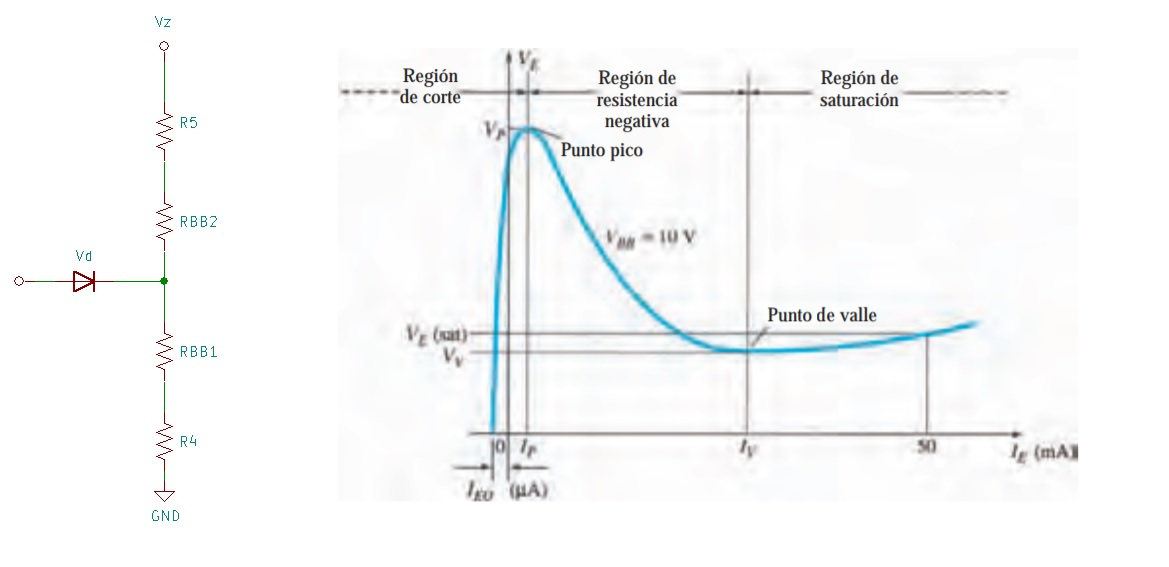
\includegraphics[width=\textwidth]{imagenes/fig3.jpg} 
	\caption{Circuito equivalente y curva característica}\label{fig:fig3}
 \end{center}
\end{figure}
%
La corriente que debe circular entre la base 2 y la base 1 debe ser mucho mayor que la requerida por el SCR, entonces

\end{document}
